
% SEP 2012 Group 13
% Software Design Document (SDD)
%
\documentclass[11pt, a4paper]{report}
\usepackage{graphicx}
\usepackage{fullpage}
\usepackage{url}
\pagestyle{headings}

%%% page parameters
\headsep = 25pt
\begin{document}
\oddsidemargin -0.5 cm
\evensidemargin -0.5 cm
\textwidth 15 cm
\topmargin -1.2 cm
\textheight 25 cm
\begin{center}

\includegraphics[scale=1.5]{./UniLogo}\\[1cm]    
\textbf{\Huge \bfseries Software Design Document}\\[1.5cm]
\textbf{\huge for}\\[0.5cm]


% Title
\textbf{ \huge Archaeology Robot }\\[0.3cm]
\textbf{ \huge Group 13 }\\[2cm]


\begin{tabular}{ |c | p{2cm} |}
	\hline
Yufeng Bai 1600095 & \\[.5cm] \hline
Dawei Geng 1219181 & \\[.5cm] \hline
Jun Chen 1206265 & \\[.5cm] \hline
Quang Khoi Nguyen 1187070  & \\[.5cm] \hline
Shikai Li 1214223 & \\[.5cm] \hline
Yunyao Yao 1203525 & \\[.5cm] \hline
Yatong Zhou 1204471 & \\[.5cm] \hline
\end{tabular}


\vfill

% Bottom of the page
Version 1.31 \\ [0.2cm]
{\large \today}

\end{center}
\tableofcontents



% Version History %

% IMPORTANT %
% Whenever you make a change to this document you MUST put an entry in below
% Must conform to firstName lastName &  date & description \\ \hline


\clearpage
\section*{Revision History}
\begin{tabular}{| l | l | l | l | }
\hline
Name				  &	Date        	&	Reason For Changes                  	  	&	Version     	\\ \hline
Dawei Geng		&	03 Sept 2012   &	Template			                    	      &	0.1 	    	  \\ \hline
Yufeng Bai		&	06 Sept 2012	  &	Chapter 7							                    &	0.2		        \\ \hline
Yufeng Bai		&	06 Sept 2012	  &	Chapter 8							                    &	0.3		        \\ \hline
Yufeng Bai		&	06 Sept 2012	  &	Chapter 9							                    &	0.4		        \\ \hline
Yufeng Bai		&	07 Sept 2012	  &	Fix the layout						                &	0.5		        \\ \hline
Jun Chen    	& 08 Sept 2012 	&	Chapter 1                  		  	        &	0.6     	    \\ \hline
Jun Chen   		&	08 Sept 2012 	&	Chapter 2                 	  			      &	0.7           \\ \hline
Yufeng Bai		&	09 Sept 2012	  &	Fix the error						                  &	0.8		        \\ \hline
Khoi Nguyen 	&	10 Sept 2012   &	Chapter 4,5             				          &	0.9     	    \\ \hline
Jun Chen			&	11 Sept 2012	  &	Chapter 3.1,3.2                	  		    &	1.0    	      \\ \hline
Yufeng Bai		&	12 Sept 2012	  &	Fix grammar and spelling errors			      &	1.1		        \\ \hline
Yatong Zhou   &	12 Sept 2012   &	Chapter 6 and error fixing				        &	1.2     	    \\ \hline
Khoi Nguyen   &	14 Sept 2012   &	Chapter 4 review                          &	1.30          \\ \hline
Yufeng Bai	&	10 Oct 2012	&	fixing SDD document				&	fixing	\\ \hline
Yufeng Bai	&	10 Oct 2012	& fixing the pictures of add	&	fixing \\ \hline
Jun Chen     		&16 Oct 2012        	&	fixing chapter 6,7,8                  	  	&	fixing   	\\ \hline
Yufeng Bai	&	16 Oct 2012		& fixing the SDD			&	fixing2 \\ \hline
Jun Chen    		&	17 Oct 2012     	&	Add state diagram and class diagram                  	  	&	fixing     	\\ \hline
Jun Chen    		&	17 Oct 2012       	&	Combining 2 fix version, layout fix.               	  	&	fixing3   	\\ \hline
Jun Chen    		&	 19 Oct 2012     	&	error fix                  	  	&	fixing3   	\\ \hline
Jun Chen      		&	22 Oct 2012       	&	spell check, making final version                  	  	&	1.31     	\\ \hline
Yufeng Bai		&   22 Oct 2012		&	Changing the diagram and relevant explanation	&	2.0 \\ \hline
%





\end{tabular}
\clearpage

% Introduction %

\chapter{Introduction}% (fold)
\label{cha:I}
%Provide an overview of the SDD and a description of the scope of the system to be developed.%


\section{Purpose and Scope}
\subsection{Purpose}
The purpose of making this Software Design Document (SDD) is to give the details of the design of the archaeology robot and its system, which is designed by our group (group 13). In this document, we will give an overall description of architectural design, system organisation and critical modules of the system. This document describes some general ideas of how do we design the system and how do we implement requirements into the system. This document will be given to the team members so that they can construct the system based on the requirements. Also this document will be used as a reference for further developments.
%Define the purpose of this document, specify intended readership of the document.%


\subsection{Scope}
The document describes the robot side, host side and some relevant details about the GUI. It is intended to give the developers and clients all specific details about how the system is constructed. This Software Design Document (SDD) is also used to give details of overall design of archaeology robot. It will contain nine parts : Introduction which will give an overall description of the design, System Overview which will show the design of the system, System Architecture and Components Design, Architectural Description which also includes alternatives and rationale, Data Design, Human Interface Design, Resource Estimates and Definitions, Acronyms and Abbreviations.
%Identify the context of the system; explain what the proposed system does (and what does not, if necessary); describe the relevant benefits, objectives and goals. The description should be consistent with your SRS.%


\section{References}
This Software Design Document (SDD) references these files below:
\begin{enumerate}

  \item Software Requirements Document (SRS) : this document demonstrate all the requirements for this project.

  \item Software Project Management Plan (SPMP) : this document shows the details of how do we manage our project.

  \item UML files : the class diagram show how do we design and implement our system.

\end{enumerate}
%Provide a complete list of all documents that you referenced in SDD.%

\pagebreak
\section{Overview}
This Software Design Document will be organised in a way that describe System, Architectural Design, GUI Design and Resource Estimates specifically and logically. \\ \\
In the beginning of the document, it will give an introduction of this document (Purpose and Scope) and System Overview. After that, the document will give some high level architectural designs of the whole system, which include System Architecture and Components Design, Architectural Description. In these parts, a explanation about the whole architecture and major component of the software and how they interact will be indicated.  Then the document will move to the Data Design part, which demonstrates the Design Details of the system. After the Data Design, it will show the design of Human Interface and Resource Estimates. In Human Interface part, the major components of GUI and their functions  will be demonstrated. In Resources Estimates, all resources which are used in the whole system will be provided. Lastly, there are some Definitions, Acronyms and Abbreviations at the end of the document. \\ \\
This document will follow the developing stages and the template of the SDD is generated according to client's requirement.
%Overview the content of the document; explain how the SDD is organized.%

\section{Constraints}
The follow restrictions, limitations, and constraints will affect the design and implementation of the system:
\begin{itemize}
  \item The robot should be set up correctly before testing.
  \item The robot is forbidden to be damaged.
  \item The robot is not allowed to go out of the map.
  \item The robot is not allowed to push the wall and colliding is not permitted.
  \item The map should be set up correctly before testing
  \item The map is in fixed size (less than A1).
  \item Pixels will be the smallest component of a map, at 25mm by 25mm.
  \item There are some no-go zones on the map.
  \item The system must has save and load function.
  \item An acceptable latency is 300ms.
  \item There are some hidden walls on the map.
  \item The robot is only allowed to  search the map by pixels on auto mode.
  \item 4 Pixels make up 1 zone on the map.
  \item The maximum speed of robot is 10 inches per second.
  \item The size of the wall is more than 3 pixels.
\end{itemize}
%Briefly describe any restrictions, limitations, and constraints that affect the design and implementation of the system.%


% chapter Introduction (end)
\pagebreak


\chapter{System Overview}% (fold)
The main goal of the system is to let the robot is able to be used for survey an archaeological site containing the remnants of an ancient city under both automated and manual control.  The robot is not allowed to be damaged during the whole working process. The hardware system is the robot who execute all detection, the software system is used to control the robot and implement information transmission between the Host and Robot. Generally, there are three mainly part for this system: the Host, the Robot and the communicator.  

\section{Robot}
The robot is used to execute the detection of the archaeology in one sized map. The map contains the objects like hidden walls and obstacles, the robot is required to detect all these objects when it searches the map. The robot has the light and ultrasonic sensor which are used to implement the detection operation.     

\section{Host}
The Host is installed on the PC and the function of the Host includes:
\begin{enumerate}
\item Using GUI to demonstrate the map, include all objects on the map and the robot states.
\item Using Navigation to implement auto and manual control, which is combined with GUI. 
\item Parse the XML file to the data structure which contains the map information.
\end{enumerate}

\section{Communication Component}
The Communication Component is used to connect the Host system with the Robot. It allows the Host to send the command to the robot and robot to send the searching information to the Host. In the whole system, the communication Component is implemented by the Bluetooth. \\ \\
The diagram of communication Component shows below:
\begin{figure}[h]
  \centering
    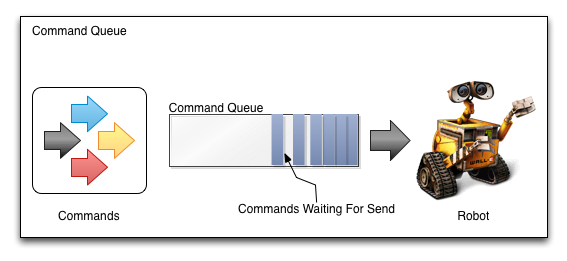
\includegraphics[width=16cm]{CommandQueue.png}
  \caption{The communication diagram}
\end{figure}
  
\pagebreak
\section{Conclusion}
In conclusion, the whole system of this project contains three parts:
\begin{itemize}
  \item Robot is the main body to implement all detection operations. It is also required to return the feedback about map and immediate robot status 
  \item Host is used to implement the controlling of the robot and demonstrate the robot status. The Host also takes responsibility to store(load) the map to(from) XML. 
  \item Communication Component is used to connect the Host with Robot. All transmission of the information has to use the communication part. 
\end{itemize}
With these three parts, the system will work properly and do the task based on the client's requirements and Project Description.

%Briefly introduce the system context and design.%


% chapter System Overview (end)
\pagebreak


\chapter{System Architecture and Components Design}% (fold)
\label{cha:SACD}
%In this section, you should cover the following content, in several subsections.%


\section{Architectural Description}
The archaeology robot system we make will have three major parts that work together to achieve the goal. These three parts are Host System, Robot System, blue-tooth Connection. The Robot System is mainly used to execute the detection, the Host System is the controlling centre which is used to control the robot and record the information from remote interface. The role of the blue-tooth Connection is to connect the Host System with Robot System. The System connection diagram display below: 
\begin{figure}[h]
  \centering
    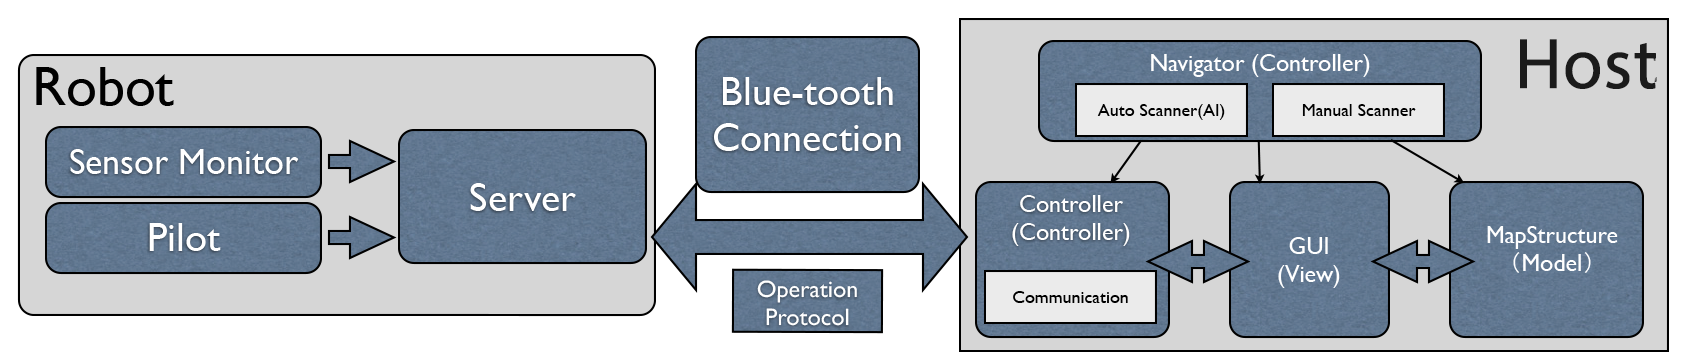
\includegraphics[width=16cm]{System.png}
  \caption{The system connection diagram}
\end{figure}
\section{Component Decomposition Description}
\subsection{Robot System}
The Robot System is installed in the archaeology robot. Basically the Robot System will be implemented all basic functionalities of the robot. Also it is required to respond to commands which are sent from the Host System. Moreover the Robot System should also include functionalities that can make the robot move according to the received command. There are three components in the Robot system:
\paragraph {Server} is used to accept the commands from Host System and send the messages to the Host System. All the messages which will send to Host System need to packet here. All commands sending from Host System also need to unpacked in this server.
\paragraph {Sensor Monitor} include light sensor and ultrasonic sensor. The light sensor is used to detect the hidden walls which will use different colour to mark on the map. The ultrasonic sensor is used to detect the obstacles on the map. As the safety priority principle, the robot is forbidden to collide the obstacle, the ultrasonic is the tool to protect the robot. In our design, when ultrasonic detects the obstacles, it will notify the robot, then robot will stop in a few distances front of the obstacle.
\paragraph {Pilot} is used to control the movement of the robot and the detection of the sensors. It is also used to control the rotation of the robot by setting the speed of robot's wheels on both sides.      


\subsection{Host System: }
The main purpose of the Host System is to implement remote controlling of robot. Following the Requirement Description, the robot is required to be controlled by users. It is necessary to build a control panel on PC, then the user is able to control the robot and check the robot status from PC. In our design, the Host System will follow the Model-View-Controller pattern. There are three main parts representing the three components of this pattern: GUI(View), MapStructure(Model), Controller and Navigator(Controller).    
\newline
\paragraph{MapStructure and XML Documents(Model)} 
\begin{enumerate}
\item MapStructure: The Map is composed by pixels. The size of each pixel is 25mmx25mm. The robot search the map using pixel as the unit. The map also need to include the information of all object like hidden walls and obstacles. In addition, some related robot status also is stored in the Map Structure(the current position and the start position of the robot).
\item XML Documents: The map is stored in the XML file. The map information is able to be checked by GUI, and the GUI also can store the map information in XML file.
\end{enumerate}
\paragraph{GUI(View)} The GUI will contain three components which are:
\begin{enumerate}
\item Main GUI: is the graphic interface for the host system which is used to show to the user. The main frame of it has many small components which is able to implement different functions. It includes buttons to control the robot(the movement, speed and mode change), robot status(battery level, current
speed and current position), system status(the bluetooth connection), save, load and create
map(the size and position of the map and no go zones, load(save) the map from(to) database)
and menu(the group introduction). 
\item Map Panel: is a component of the GUI that shows the surveying map. It is used to display
the location of the robot and draw the real map into it, which means the map panel will display
and draw everything the robot explored. After the survey, the map viewer will save the map
into the database if it receives a 'save' command from the host. The map panel also contains
the icon of the map, different colour represents different object on the map, for example, the
red colour represents the no-go zones, the black colour represents unexplored area.
\item Information Window: All operation for the GUI will display on the Information window,
also the Information window shows the brief introduction of every group member.
\end{enumerate}
%Describe the architectural design of the whole system. Typically, you should include a block diagram showing the major subsystems and their interconnec- tions.%
\paragraph{Controller and Navigator(Controller)}
\begin{enumerate}
\item Controller: The controller takes responsibility to connect with the robot, the function of controller is similar with the Server, its main function is packeting the commands which send from Host System to Robot System and unpacking  the messages which receive from the Robot System.
\item Navigator: The Navigator has two component, the Auto Scanner and the Manual Scanner. The main function of Navigator is to make the algorithm to control the robot scan the map on auto and manual scan modes. In Auto-scan mode, the Navigator will make the algorithm to let the robot to find path automatically and send all objects of the map to the Host System. On Manual-scan Mode, the Robot is controlled by the user. The user is able to send the command to control the movement of the robot. The safety is priority for both mode, the Navigator is forbidden the user to execute some unsafe operation. For example, if user wants the robot to collide the obstacles or the user wants the robot to access the no go zones, the robot will not move follow the commands. The Navigator is combined with  the GUI.    
\end{enumerate}
\subsection{Blue-tooth Connection}
The bluetooth is used to connecting the Host System with the Robot System. All the information transmission need to go through the bluetooth, the bluetooth is wireless so that it will not limit the move range of the robot.   



\section{Detailed Components Design Description}
\subsection{Host}
\subsubsection{GUI}
\begin{enumerate}
\item Component Identifier: C-0
\item Purpose: GUI is a interaction between the host and the robot. GUI is able to send the host's command to the robot and get the feedback from the robot.  
\item Function: It provides the GUI for the Host, which is convenient for Host to control the robot. For example, the Host can control the movement, speed, and the searching mode of the robot. The GUI is also able to display the feedback from the searching of the robot, for example, the GUI can display the hidden walls or obstacles of the map. Basically, GUI takes responsibility to translate the Host's command to robot instruction and translate the robot feedback to Host message, then send between the robot and host.   
\item Subordinates: LEGOGUI, CommandTranslator, About, MainControlThread, Operation, TextAreaPrintStream. 
\item Dependencies: MapStructure, Navigation
\item Interfaces: Host
\item Data: None
\end{enumerate}

\subsubsection{MapStructure}
\begin{enumerate}
\item Component Identifier: C-1
\item Purpose: The map structure is used to build the map for the robot. The robot need to search in a sized map. The map needs to display on the map. 
\item Function: The map is made by pixels, the robot is required to search on the map and map also contains some information of the robot(the current and start position of the robot), as a result, the robot status and some relevant operations of robot also are required to connect with map.
\item Subordinate: Map, Operation, Pixel, RobotStatus
\item Dependencies: XMLDocuments
\item Interface: Host
\item Data: Contain the current and start position of the robot. 
\end{enumerate}

\subsubsection{Navigation}
\begin{enumerate}
\item Component Identifier: C-2
\item Purpose: The navigation is used to control the robot. Robot is required to search and find all objects on the map in auto and manual mode, it is necessary to use navigation to control the searching of the robot. The navigation also contains the algorithm to define scan trace of the robot. 
\item Function: The function of the navigation is to control the movement and scan of the robot. When the robot is in auto mode, the robot is able to scan the map and find all objects automatically. When the robot is in manual mode, the robot is required to be controlled by Host, Host is able to give the command to the robot, then robot executes the operation according to the instruction from host. The pathfinder is a method to define how the robot scan the map. 
\item Subordinate: AutoNavigation, ManualNavigation, PathFinder, RobotAutoScanner, RobotManualScanner, RobotNavigator
\item Dependencies: MapStructure
\item Interface:Host
\item Data: None
\end{enumerate}

\subsubsection{XMLDocuments}
\begin{enumerate}
\item Component Identifier: C-3
\item Purpose: According to the client requirement, the map and the relevant information need to store in the XML file. 
\item Function: The function of the XMLDocuments is to create the xml file to store the map information and load the map information from the XML file. 
\item Subordinate: XMLDocuments, XMLReaderWriter
\item Dependencies: MapStructure
\item Interface: Host
\item Data: Contain the map information.
\end{enumerate}

\subsection{Robot}
\begin{enumerate}
\item Component Identifier: C-4
\item Purpose: The Robot is required to do the relevant operation on the actual map, the Robot is used to implement the movement, detection, robot state monitoring and sensor monitoring on Auto mode and Manual mode. The robot is also required to handle some safety situation include it has to stop automatically in some circumstance. 
\item Function: The Robot contains the methods to implement the basic operation of the robot. In our design, we use different value to represent different operation, for example, ``0x000'' represents the forward pressed, which is more convenient for us to implement all function. Since the map is made by pixels, the robot will move use pixel as unit. The robot side also includes the function to monitor the sensor. The robot has light sensor and ultrasonic sensor, light sensor is used to detect the hidden wall and ultrasonic is used to detect the obstacles. The robot is required to use ultrasonic sensor to find the obstacle and avoid to collide the obstacles. In the sensor design part, it is necessary to stop the robot immediately in some danger situation no matter which mode the robot is.      
\item Subordinate: BTRobotDriver, Operation, Robot, SensorMonitor.
\item Dependencies: None
\item Interface: Robot 
\item Data: the different data represents different operation of the robot.  
\end{enumerate}

\subsection{Class Files}
\subsubsection{GUI-LEGOGUI}
\begin{enumerate}
\item Component Identifier: C-5
\item Purpose: LEGOGUI is used to generate the main GUI. 
\item Function: The LEGOGUI is used to build the main GUI, include the size and the layout of the GUI. The LEGOGUI defines the different panel of the GUI, the position of these panels and the size of these panels. This class also build the connection between the GUI and database.
\item Dependencies: TextAreaPrintStream, About, CommandTranslator
\item File: GUI
\item Data: Node
\end{enumerate}

\subsubsection{GUI-TextAreaPrintStream}
\begin{enumerate}
\item Component Identifier: C-6
\item Purpose: GUI need to receive the input message
\item Function: This class is used to get the message from the input, write these message to GUI and then print all these messages out, which is a part of the GUI
\item Dependencies: None
\item File: GUI
\item Data: Receive the data from the input and  write them to GUI, then print them out.
\end{enumerate} 

\subsection{GUI-About}
\begin{enumerate}
\item Component Identifier: C-7
\item Purpose: GUI is required to contain some Group introduction.
\item Function: This class is used to build a window to display some group information, for example, the Group name and the team members' names. The About class also has the contact method.
\item Dependencies: None
\item File: GUI
\item Data: the introduction message.
\end{enumerate}

\subsection{GUI-CommandTranslator}
\begin{enumerate}
\item Component Identifier: C-8
\item Purpose: GUI works as a controller which connect the host with robot. It is required to translate the user's input to the command which is able to be read by GUI. 
\item Function: Basically, different number represents different input command, for example, the number 1 represents the input command `` f '', which is able to be read by GUI. The user can input the command by GUI. 
\item Dependencies: Node
\item File: GUI
\item Data: the numbers which represent different operation.
\end{enumerate}

\subsection{GUI-MainCntrolThread}
\begin{enumerate}
\item Component Identifier: C-9
\item Purpose: The GUI need to connect with the robot and control it.
\item Function: In our design, it is required to use bluetooth to connect the robot, the connection function is from lejos API, then the GUI is able to use InputStream and OutStream function to input the command to the robot, different number represents different command. When connection is successful, when the user input different string, the robot will read the relevant number, then do the corresponding operation.   
\item Dependencies: None
\item File: GUI
\item Data: the string as command input by user and the numbers which represent different command. 
\end{enumerate}

\subsection{GUI, MapStructure, Navigation, Robot-Operations}
\begin{enumerate}
\item Component Identifier: C-10
\item Purpose: Collect different number to represent different command
\item Function: Display the relevant numbers which is used for the system
\item Dependencies: None
\item File: GUI, MapStructure, Navigation, Robot
\item Data: the relevant numbers which represent different operation
\end{enumerate}

\subsection{MapStructure-Map}
\begin{enumerate}
\item Component Identifier: C-11
\item Purpose: The GUI need to contain a map to demonstrate the searching of the robot. 
\item Function: This class generates the map by pixel, it also demonstrate the position of the robot, which includes the current position and start position. In addition, this class defines the layout of the no-go zones.
\item Dependencies: Pixel
\item File: MapStructure
\item Data: the input data which is used to define the size of the map, and the position of the robot.
\end{enumerate}

\subsection{MapStructure-Pixel}
\begin{enumerate}
\item Component Identifier: C-12
\item Purpose: Since the map is made by pixels, it is necessary to define the pixel.
\item Function: This class defined the specific parameters for each pixel, which contains the size of one pixel and the size of different object. For example, the smallest hidden wall's size is one pixels.
\item Dependencies: None
\item File: MapStructure
\item Data: the specific number represents the size of different object.
\end{enumerate}

\subsection{MapStructure-RobotStatus}
\begin{enumerate}
\item Component Identifier: C-13
\item Purpose: Some robot information is required to store on the map.
\item Function: The class defines the specific location of the robot.
\item Dependencies: Pixel
\item File: MapStructure
\item Data: None
\end{enumerate}

\subsection{Navigation-AutoNavigation, RobotAutoScanner}
\begin{enumerate}
\item Component Identifier: C-14
\item Purpose: Implement the auto mode of the robot, which is required robot to move and detect automatically on the premise of safety.
\item Function: Using PathFinder class to let the robot scan the whole map automatically, the robot need to record the current position of the robot and the path from start position to current position. The robot also is required to find the path from current position to nearest unexplored Pixel.
\item Dependencies: Map, PathFinder, Pixel, RobotNavigator
\item File: Navigation
\item Data: None
\end{enumerate}

\subsection{Navigation-ManualNavigation, RobotManualScanner}
\begin{enumerate}
\item Component Identifier: C-15
\item Purpose: Implement the manual mode of the robot, which is required robot to move and detect by the controlling of the user via GUI on the premise of safety.
\item Function: The robot need to receive the commands from GUI. In our design, we will use one queue to receive the command from host machine, the scan method is also from PathFiner class. The different direction also use different value to represent.
\item Dependencies: Map, PathFinder, Pixel, RobotNavigator
\item File: Navigation
\item Data: None
\end{enumerate}

\subsection{Navigation-PathFinder}
\begin{enumerate}
\item Component Identifier: C-16
\item Purpose: It is necessary to define one algorithm to let robot scan all pixels of the map.
\item Function: Firstly, Using Depth First Search to traverse all pixels in the map. The robot decides whether the robot finish the traverse or not according to the return value of the DFS. Second, Using PathFinder function to find the path from the current position to next position. Thirdly, Using findNearestUnexplorePixel function to find the nearest unexplored pixel when the 4
directions(east, west, north, south) of the current position have already explored. Finally, Using Robot Scanner class to decide when and how the robot moves.
\item Dependencies: Map, Pixel, RobotNavigator
\item File: Navigation
\item Data: None
\end{enumerate}

\subsection{Navigation-RobotNavigator}
\begin{enumerate}
\item Component Identifier: C-17
\item Purpose: The robotNavigator is a class to implement robot and read all messages from map it is a unify class to let the robot detects following the design. 
\item Function: The robotNavigator is able to control the movement of robot and detect all objects, and translate the GUI command to Robot instruction.   
\item Dependencies: Map, Pixel, MainControlhread
\item File: Navigation
\item Data: the number which represents different command.
\end{enumerate}

\subsection{XMLDocuments-XMLDocument, XMLReaderWriter}
\begin{enumerate}
\item Component Identifier: C-18
\item Purpose: According to the clients requirement, the map and the relevant information need to store in the XML file. 
\item Function: Define the method to create a XML file to save the new map, and another method to load the map from XML file.
\item Dependencies: Map
\item File: XMLDocuments
\item Data: None
\end{enumerate}

\subsection{Robot-BTRobotDriver}
\begin{enumerate}
\item Component Identifier: C-19
\item Purpose: The unify class to implement all functions of the robot, include the bluetooth connection and the sensor monitoring.
\item Function: The function of this class includes connect the host machine with robot, and receive the command from the host machine. The robot is able to move following the command from host machine. All sensors' functions are also able to implement in this class. 
\item Dependencies: BTConnection, Robot,
\item File: Robot
\item Data: the numbers which represent different command.
\end{enumerate}

\subsection{Robot-Robot}
\begin{enumerate}
\item Component Identifier: C-20
\item Purpose: Collect all operation of the robot, include the movement and stop in manual and auto mode
\item Function: The Robot is required to control the robot move forward, backward, rotate and stop in auto and manual mode.
\item Dependencies: None
\item File: Robot
\item Data: None
\end{enumerate}

\subsection{Robot-sensorMonitor}
\begin{enumerate}
\item Component Identifier: C-21
\item Purpose: It is necessary to build  a Thread that monitor the ultrasonic sensor when moving to avoid near walls. 
 \item Function: This class is using sensor to detect all object from the map, this function contains when the robot is need to stop and the range of the monitoring.
\item Dependencies: Robot
\item File: Robot
\item Data: None
\end{enumerate}



\section{Architectural Alternatives}
%Discuss briefly other architectures that were considered if any.%
The other alternative design which is considered is letting the robot do the exploration without
waiting command from the host system. The idea is shelved because the robot's resource is not capable
of performing the  algorithm.\\ \\
Another architecture we considered was the Object Oriented model. The Java is a object oriented model, meanwhile, the program of the system mainly use java language. OOM is a effective way to use. This model is helpful to let every developer understand each other's work content and process. However, the robot is required to terminate at any time, as the result, this model is not work well effectively. That is the reason why we abandon this model.



\section{Design Rationale}
%Discuss the rationale on selecting the architecture described in 3.1, including the critical issues and trade-off that were considered.%
The design of the system is layer architecture. The model is chosen for its support of separation
and independence. The development is spread across teams with each team being responsible
for a different part. The use of interface allows smooth integration without risk of
 incompatible method calls. If there is change in the interface, only the adjacent layer is affected
 so change is localised.

% chapter System Architecture and Components Design (end)
\pagebreak


\chapter{Data Design}% (fold)
\label{cha:DD1}
%You should cover database description and data structures in this section.%

\section{Database Description}
%Describe briefly the database(s) that is part of the system.%
The map is represented in XML format. It is created when the robot starts to explore.The map updates every time when the robot explores an area, detects
a hidden wall or an obstacle of the survey area. The information which is stored in the array is translated
and saved into XML. The XML file can be loaded as well. The detailed functionalities are
as follow:

\paragraph{Creating a map}

The map need to has width, height and coordinates of border. The size of the map is stored as digital number and the coordinates of the border are stored in an array list.

\paragraph{Recording the features of the area}

\begin{itemize}
\item  Clear Area: containing no features and is considered to be safe. The status and coordinate is saved if the area is explored.
\item	 Hidden Wall Area: containing hidden walls.The status and coordinate is saved if the area is explored.
\item  Obstacle Area: containing obstacle.The status and coordinate is saved if the area is explored.
\item  No-go-zone area: the robot is not permitted to enter the area. The status and coordinate is entered by the user.
\end{itemize}

\paragraph{Recording the position of the robot}

The coordinates of current position are stored in an array list and are flagged as visited.

\paragraph{Saving}

The map which is explored so far can be saved.

\paragraph{Loading}

The previous map can be loaded.


\section{Data Structures}
%Give the detailed design of the database, i.e., entities and their relationships. You can use either ER model or UML for this purpose.
 \begin{center}
 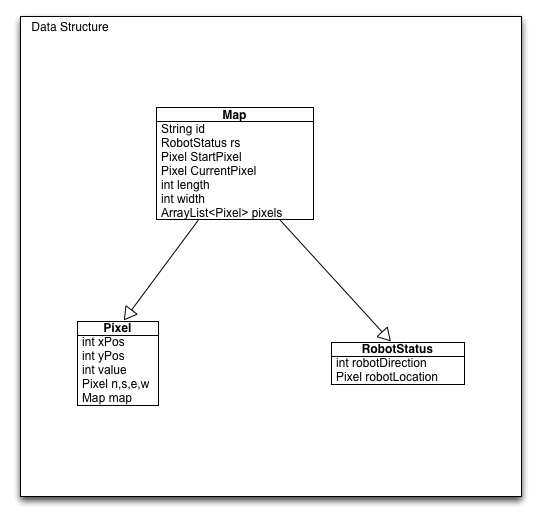
\includegraphics[width=12.20cm]{DataStructures.png}
\end{center}
\begin{center}
\textbf {Figure 4.1: Data Structure} \\[0.3cm]
\end{center}
The underlying data structure of the map database is a two dimensional array. Each element
is the pixel's information, which is indexed by its coordinating in the map. Each zone(grid)
consisted of the information of its 4 sub-grids, which is stored in a two-by-two array.
% chapter Data Design (end)

\chapter{Design Details}% (fold)
\label{cha:DD2}
%You shall describe your design by using the following diagrams to reflect all the major requirements that you documented in the SRS.%

\section{Class Diagrams}
%Describe all class diagrams that are considered in the system. Give the details (e.g., attributes, operations) associated with the class.%
The class diagrams contain four major components, the Controller diagram, GUI diagram, Navigation diagram and Robot diagram.\\ \\
The controller is responsible for the communication between the robot and the GUI(host system).  The controller allows the host system communicate with the robot by sending commands. The user can send commands from the GUI to the robot also the GUI can receive information from the robot.\\ \\
The GUI is responsible for letting the user to control the robot on host system. The GUI shows everything related to the robot and the result map that robot surveyed. Also the user can change the setting of the robot via GUI.\\ \\
The navigation is responsible for controlling the way that the robot should go. The navigation will guide the robot to go the right way and map out the map between auto mode and manual control mode. \\ \\
The robot(class) is responsible for the basic implementation of the robot. The robot(class) contains basic status of the robot and the default operations of the robot which are used to communicate with the GUI via controller.

\subsection{Controller diagram}
 \begin{center}
 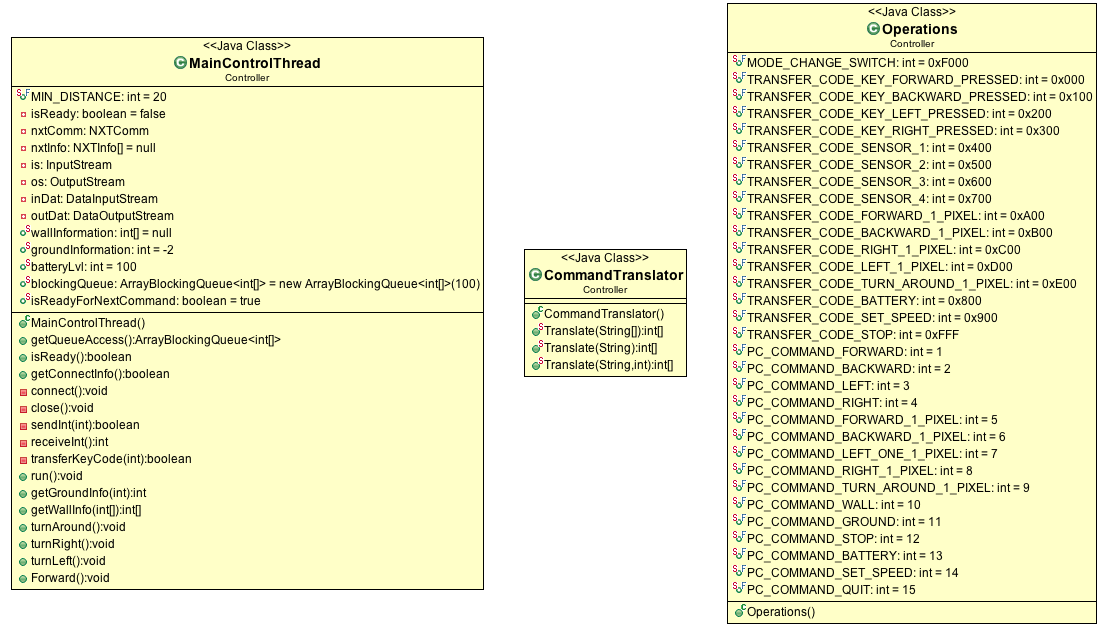
\includegraphics[width=18.20cm]{Controller.png}
\end{center}
\begin{center}
\textbf {Figure 5.1: Controller Diagram} \\[0.3cm]
\end{center}
The Controller diagram contains three parts: Operations, CommandTranslator and MainControl thread. The Operation is used to store all default operations for both the robot and the host system. The Command Translator is used to translate the commands which are sent from host system so that the robot can act as the commands tell. The MainControThread is used to communicate between the robot and the host system(sending commands).
\pagebreak
\subsection{GUI diagram}
 \begin{center}
 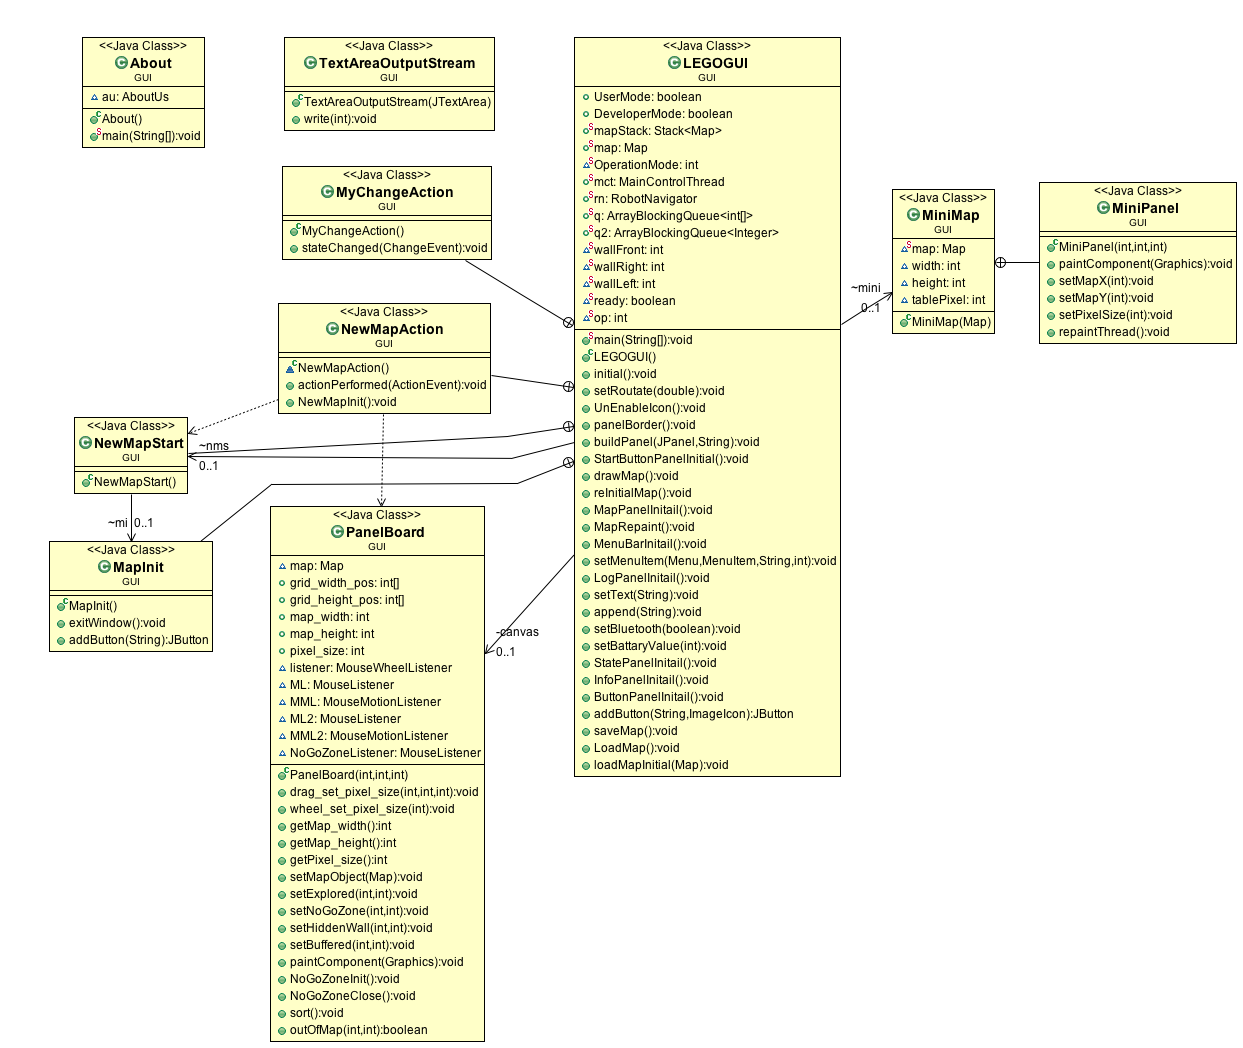
\includegraphics[width=18.20cm]{GUI.png}
\end{center}
\begin{center}
\textbf {Figure 5.2: GUI Diagram} \\[0.3cm]
\end{center}
The GUI diagram contains many classes. The GUI can be used to show the team information, create new map(set the size of the map), save map, load map, set ``no-go'' zone. show the status of the robot, change the setting of the robot(mode, speed) and connect the robot with the host system. 
\pagebreak
\subsection{Navigation diagram}
 \begin{center}
 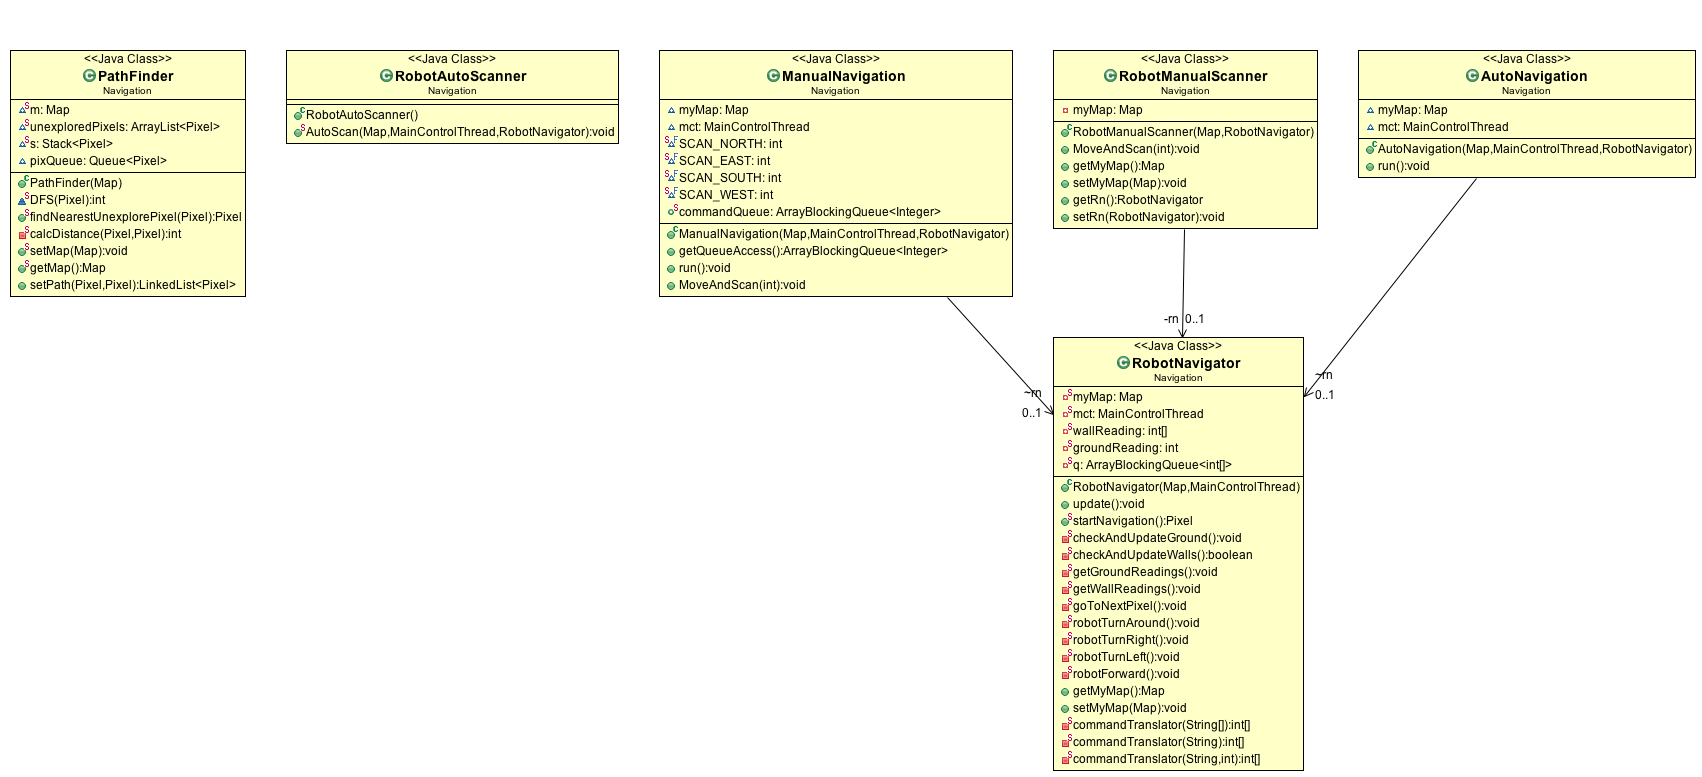
\includegraphics[width=18.20cm]{Navigation.png}
\end{center}
\begin{center}
\textbf {Figure 5.3: Navigation Diagram} \\[0.3cm]
\end{center}
For the Navigation part, the class PanthFinder has algorithm which provide path for all the scan operations. Two Navigation classes use the path found by PathFinder and then send it to the robot in auto-scan mode and manual-scan mode. The robot will move and scan the map based on the command that Navigation send. The RobotAutoScanner allows the scan operation work automatically. The RobotManualScanner allows the scan operation work manually.
\pagebreak
\subsection{Robot diagram}
 \begin{center}
 
\includegraphics[width=18.20cm]{Robot.png}
\end{center}
\begin{center}
\textbf {Figure 5.4: Robot Diagram} \\[0.3cm]
\end{center}
The robot diagram has 4 parts: Robot, BluetoothServer, SensorMonitor and Operations. The Robot class is used to store the basic information of the robot which include robot movement, robot status and scan functions. The BluetoothServer is used to connect the robot with the host system and then send back information to the host system. The operations is used to store default operation protocols for the robot. 
\pagebreak

\section{State Diagrams}
%Present the state diagrams of objects involved.%
The state diagrams will cover three major components which include robot state diagram, robot auto scan state diagram and  robot manual control state diagram. For the robot state diagram, it shows the basic states of the robot. The robot auto scan state diagram shows the states of the robot in auto-scan mode. For the robot manual control state diagram, it shows the states of actions of the robot in manual control mode.

\subsection{Robot State Diagram}
Since the robot state diagram is used to describe the basic states of the robot, the initial state of the robot is ``Not Connected''.  The robot will stay at ``Not Connected'' state and wait for any inputs until the user connect the robot with the host system via blue-tooth. When the robot is connected, the control mode will be set to manual mode, which means the robot will stay at ``Manual Mode'' state. After that, the user can change the control mode of the robot between manual mode and auto mode. Moreover, if the robot loss connection at any states, it would go back to the ``Not Connected'' state.
 \begin{center}
 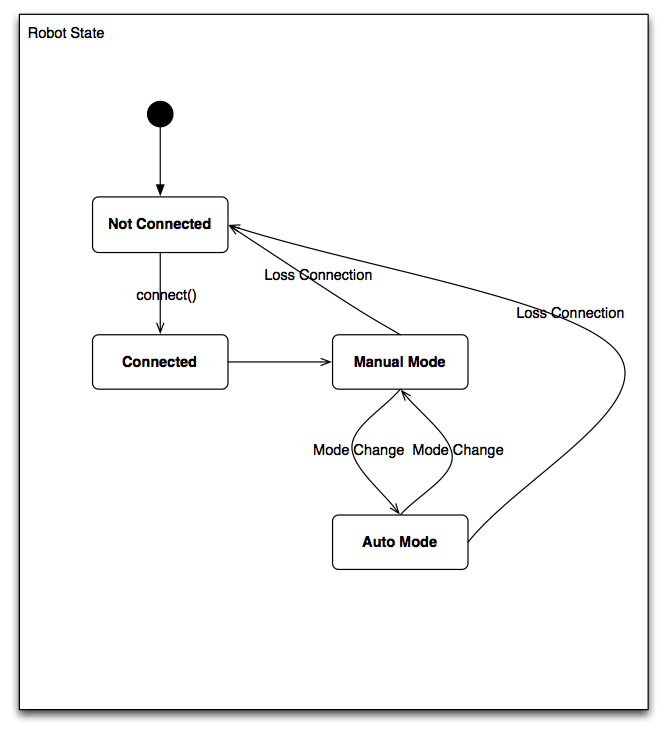
\includegraphics[width=13.20cm]{RobotState.png}
\end{center}
\begin{center}
\textbf {Figure 5.5: Robot state diagram} \\[0.3cm]
\end{center}
\pagebreak

\subsection{ Robot Auto Scan State Diagram}
When the robot is connected and in auto-scan mode, the initial state of the robot will be ``Current Pixel'' state.Once the robot stay at ``current pixel'', it will go North/West/East/South base on the navigation and pathfinder. When the robot reach the next pixel, if the pixel is explored, then robot would go back to ``Current Pixel'' state and go to next pixel again. If the pixel is not explored, then the robot will use its light sensor to scan ground and then Scan all-around. After these actions finish, the robot will go back to the ``Current Pixel'' state and keep going until all pixels in the map are explored.
 \begin{center}
 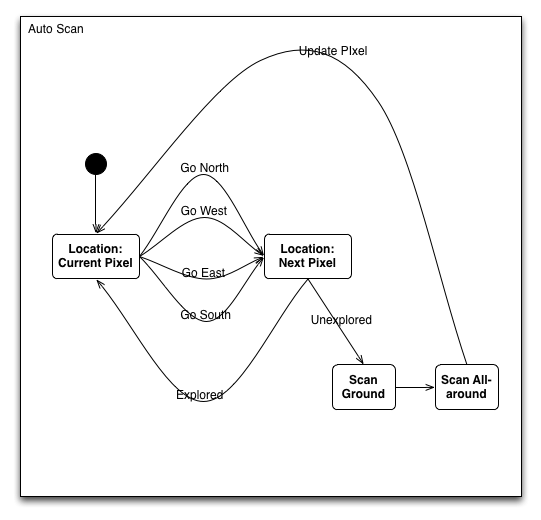
\includegraphics[width=13.20cm]{AutoScan.png}
\end{center}
\begin{center}
\textbf {Figure 5.6:  Robot auto scan diagram} \\[0.3cm]
\end{center}
\pagebreak

\subsection{  Robot Manual Control State Diagram}
When the robot is connected and in manual control mode, the initial state of the robot will be ``Stop'' state because the robot is waiting any inputs from the user via GUI interface. The GUI has six buttons for robot movement so that there are another six states in this diagram (seven in total).  When the user keep pressing the forward button, the robot will stay at ``Forward'' state and move forward. Once the user release the forward button, the robot will stop and back to ``Stop'' state. Moreover, if the ultrasonic sensor detects any walls in front of the robot, it will also stop moving forward and back to ``Stop'' state. The ``Backward'' state, ``Left'' state and ``Right'' state has the same mechanism as ``Forward'' state has. For the rest of the states, if the user press turn left/right 90 degrees button, the robot will turn left/right 90 degrees automatically and then stop, which means the robot will stay at ``Left 90 degrees''/``Right 90 degrees'' during the action of the robot. When the robot is stop, it will go back to the ``Stop'' state.
 \begin{center}
 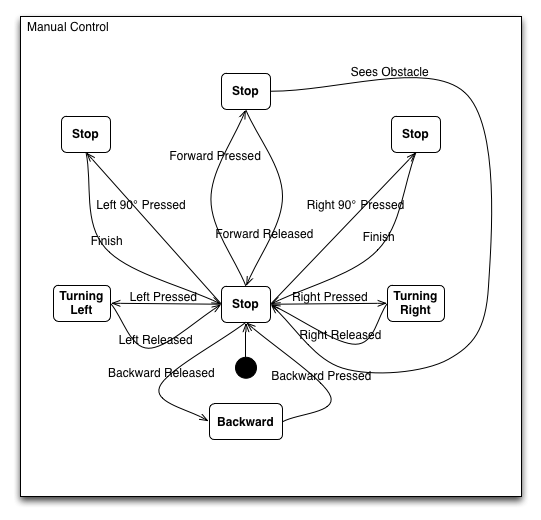
\includegraphics[width=13.20cm]{RobotManualControl.png}
\end{center}
\begin{center}
\textbf {Figure 5.7: Controller state diagram} \\[0.3cm]
\end{center}
\pagebreak


\section{Use Case Diagrams}
%Present the state diagrams of objects involved.%
\begin{figure}[h]
  \centering
    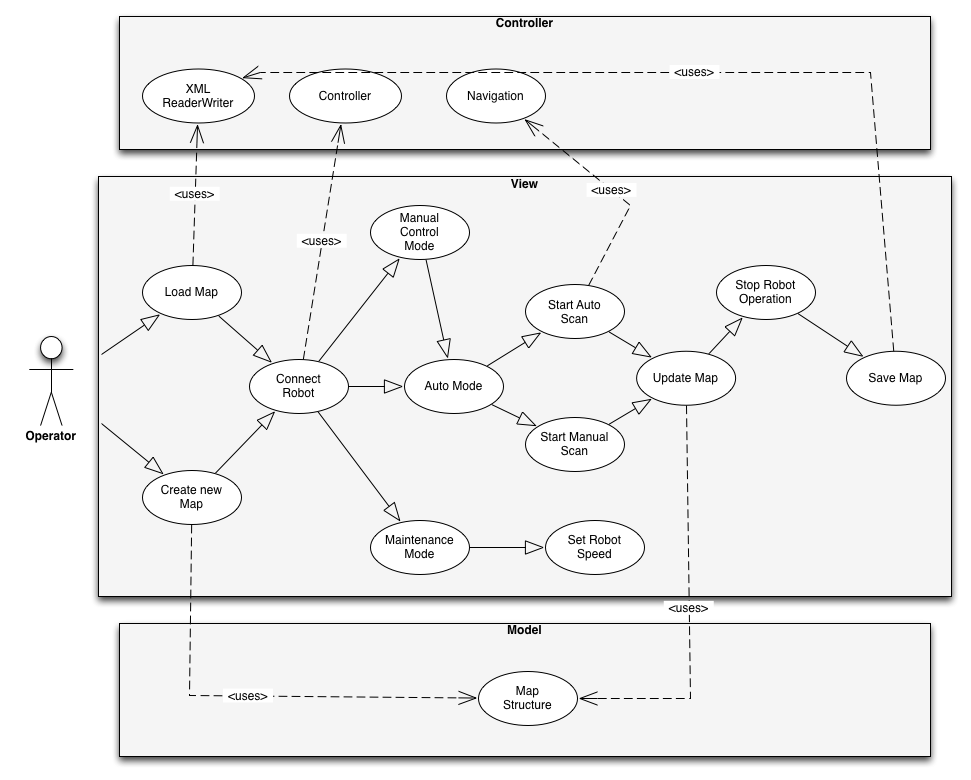
\includegraphics[width=16cm]{UseCase.png}
  \caption{Use Case Diagram}
\end{figure}
The use case diagram above shows all the cases that user can operate on the graphic user interface. The user is allow to load the map from XML file or create the new map on GUI. \\ \\
When user chooses to create the new map, user is  allowed to set initial value of map like map height, weight and start coordinate. Then operator is able to connect the robot and do the further operation such as auto scan, manual scan, change the robot speed and change to the maintenance mode. In addition, the operator is able to call the controller to implement navigation functions. The map on the map will update synchronously. The operator is also allowed to save the map at any time.  \\ \\ 
When user chooses to load the map from XML files, the operator is able to get one map from XML file, the other operation is the same as the situation when user chooses create new map.
\newpage


\section{Interaction Diagrams}
%Present the interactions of objects involved.%
%Note: all the diagrams shall be numbered and link to the requirements in%
%the SRS; UML notations should be strictly followed.%
\subsection{Interaction Diagram: Open and Connect Robot}
\begin{figure}[h]
  \centering
    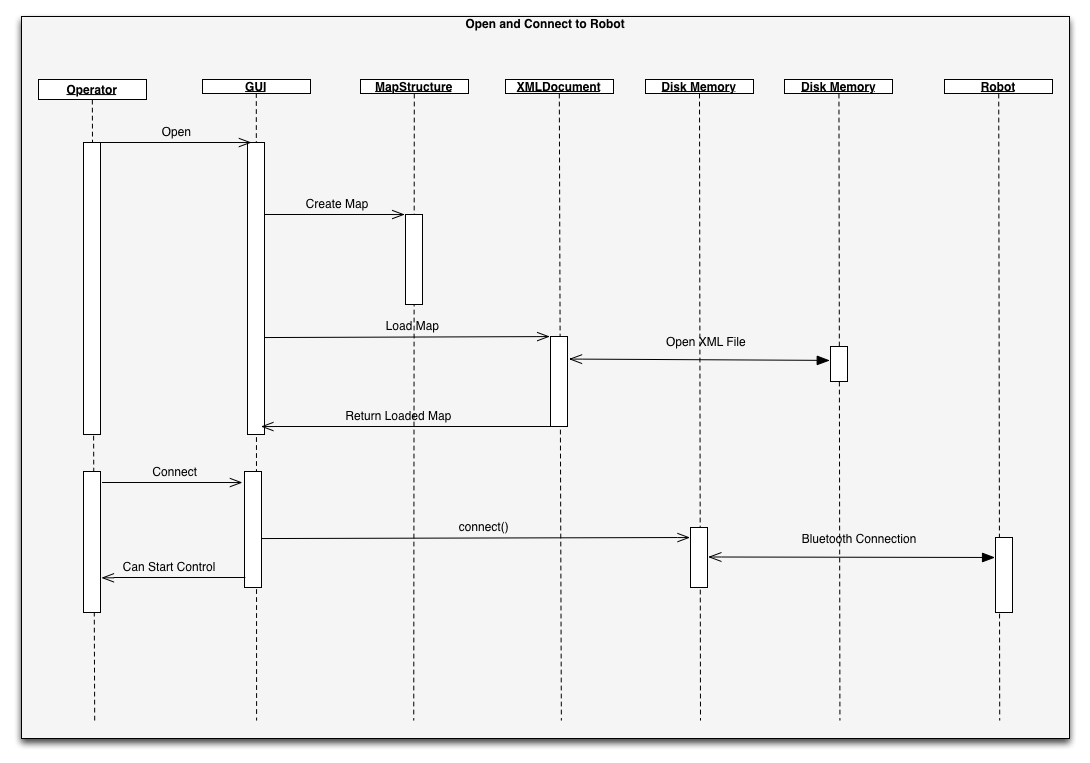
\includegraphics[width=16cm]{Seq1.png}
  \caption{Open and Connect Robot}
\end{figure}
The above diagram demonstrates how the operator opens GUI, load(create) the map and connects the Robot.
\\ \\ The operator opens the GUI, then operator is able to choose to create map or load map. If the operator chooses to create the map, the map will build according to the map structure functions. If the operator chooses to load the map, the map is able to be loaded from XML document. 
\\When the operator creates or loads the map,  the GUI is able to open the XML file and connect the robot by bluetooth. \\ \\
After the connection successfully, the GUI will give a response to the operator, then operator is able to control the robot. 
\pagebreak
\subsection{Interaction Diagram: Control the Robot in Manual Control and Auto Scan}
\begin{figure}[h]
  \centering
    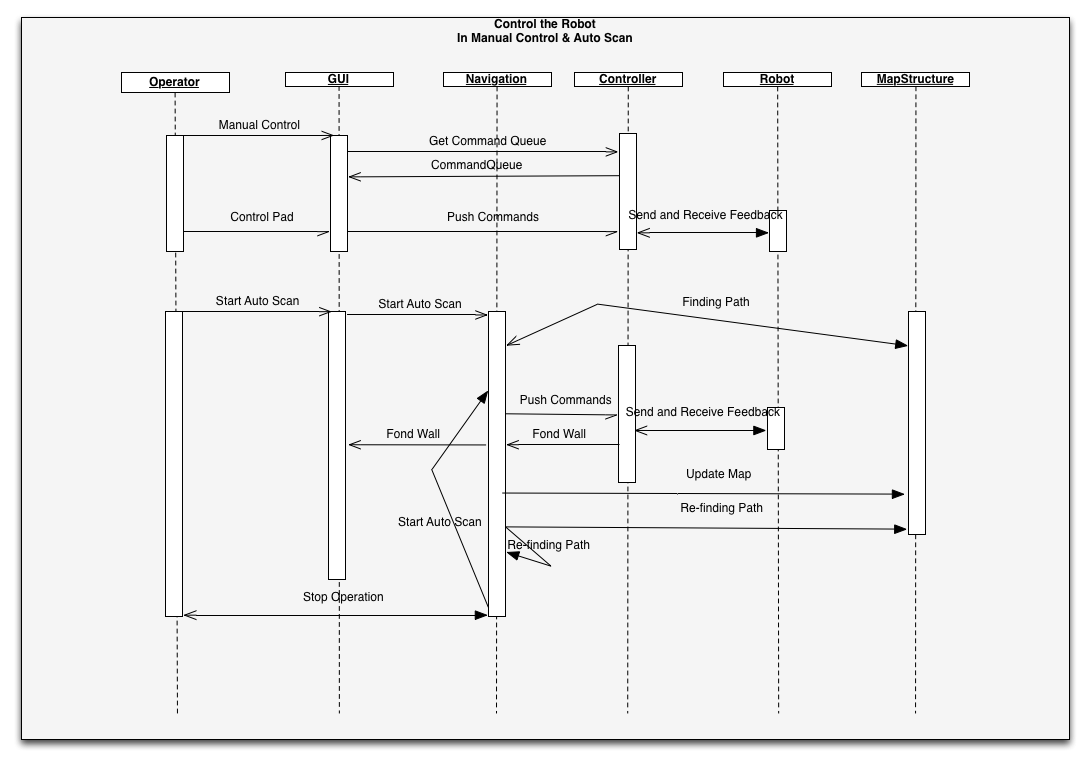
\includegraphics[width=16cm]{Seq2.png}
  \caption{Control the Robot in Manual Control and Auto Scan}
\end{figure}
The above diagram demonstrates the robot controlling in manual control and auto scan.\\ \\
In manual control, operator is allowed to send the command to the commandQueue via GUI, then robot is able to receive the commands from the controller. Also, the robot is able to send the feedback to the GUI via Controller.\\ \\
When the operator choose the mode to auto scan, then the robot can start auto scan by using the functions from navigation. The functions of  Navigation include to find the hidden wall, find the obstacles and find the path. Meanwhile, the map will update synchronously.\\ \\
The operator also is allowed to stop the scan operation at any time.    
% chapter Design Details (end)
\pagebreak
\subsection{Interaction Diagram: Control the Robot in Manual Scan}
\begin{figure}[h]
  \centering
    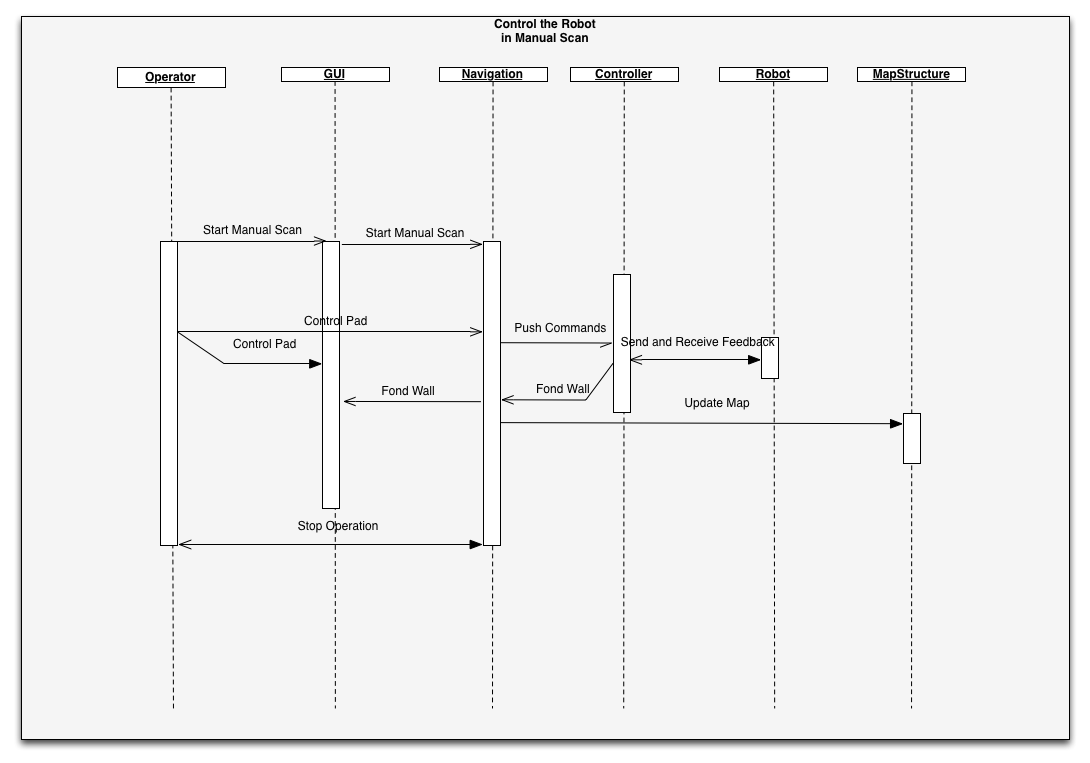
\includegraphics[width=16cm]{Seq3.png}
  \caption{Control the Robot in Manual Scan}
\end{figure}
The above diagram demonstrates the robot controlling in Manual Scan.\\ \\
In Manual Scan, operator is allowed to send the command to the commandQueue via GUI, then robot is able to receive the commands from the controller. Also, the robot is able to send the feedback to the GUI via Controller. Then the robot can start manual scan by using the functions from navigation. The functions of  Navigation include to find the hidden wall, find the obstacles and find the path. Meanwhile, the map will update synchronously.\\ \\
The operator also is allowed to stop the scan operation at any time.    
% chapter Design Details (end)
\pagebreak
\subsection{Interaction Diagram: Save Map and Editing No-go Zone}
\begin{figure}[h]
  \centering
    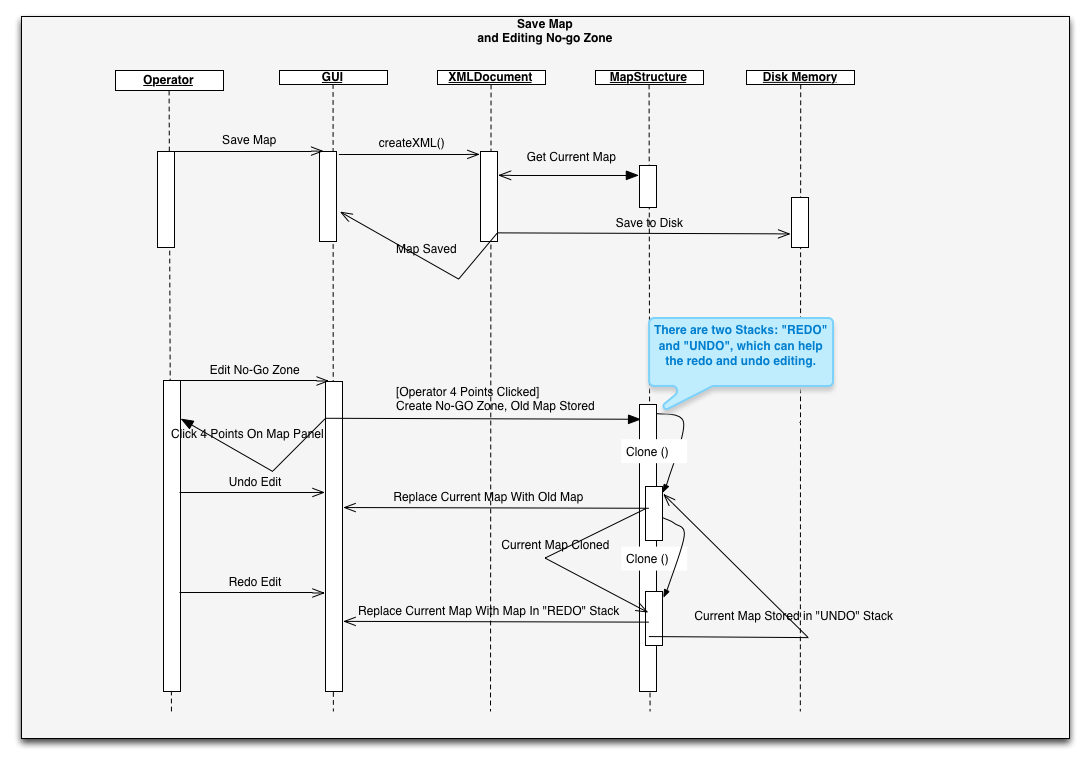
\includegraphics[width=16cm]{Seq4.png}
  \caption{Save Map and Editing No-go zone}
\end{figure}
The above diagram demonstrates the operation about saving map and editing No-go zone. \\ \\
The operator is able to save map on GUI. GUI can implement the createXML function to save the map in XMLDocument. Then savehte XML file in the disk memory. \\ \\
The operator also can edit the no-go zone. When operator wants to edit no-go zone by GUI, the new no-go zone will be clone to the current map. Then the new map will be displayed on the GUI. Operator also is allowed to implement ``redo'' and ``undo'' operation.\\ \\
The new map will be displayed on the GUI.


\chapter{Human Interface Design}% (fold)
\label{cha:HID}

\section{Overview of the User Interface}
%Describe briefly the general functionalities of the system from end users? per- spective.%
The Graphical User Interface is used to communicate with the robot. The GUI is connected with robot, the user is able to control the robot by GUI. When the robot finishes its task, the user is allowed to switch off and disconnect with robot. In addition, the GUI demonstrates the status of the robot. The status includes the speed, the power and the location of the robot. The GUI also shows the obstacles, the "no-go" zone and hidden walls, which is able to be checked on the map window.\\

The GUI is able to demonstrate the follow functions for users:
\begin{itemize}
\item Create a new map file.
\item Save maps to a XML file
\item Load maps from a XML file
\item Change the control mode (Auto or manual)
\item Connect to the robot via Bluetooth
\item Demonstrate the Blue-tooth connection status and Battery status
\item Control the moving direction of the robot(i.e. forward, backward, rotating)
\item Demonstrate the Icon of the map
\item Demonstrate the Log Information
\item Change the speed of the robot
\item Demonstrate the coordinate of the robot
\item Add "no-go" zones to the map
\end{itemize}
The GUI is displayed below:
\pagebreak
\begin{center}
 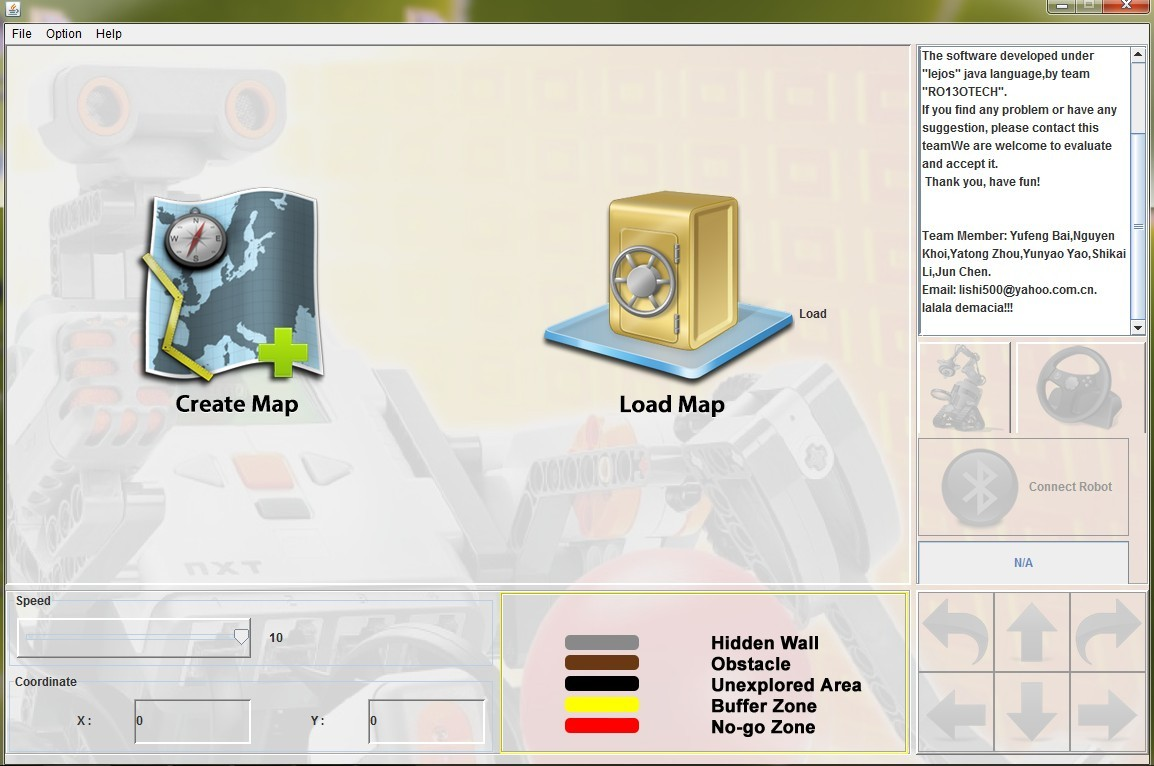
\includegraphics[width=11.20cm]{GUI_Initial.jpg}
\end{center}
\begin{center}
\textbf {Figure 6.1: GUI} \\[0.3cm]
\end{center}
\begin{center}
 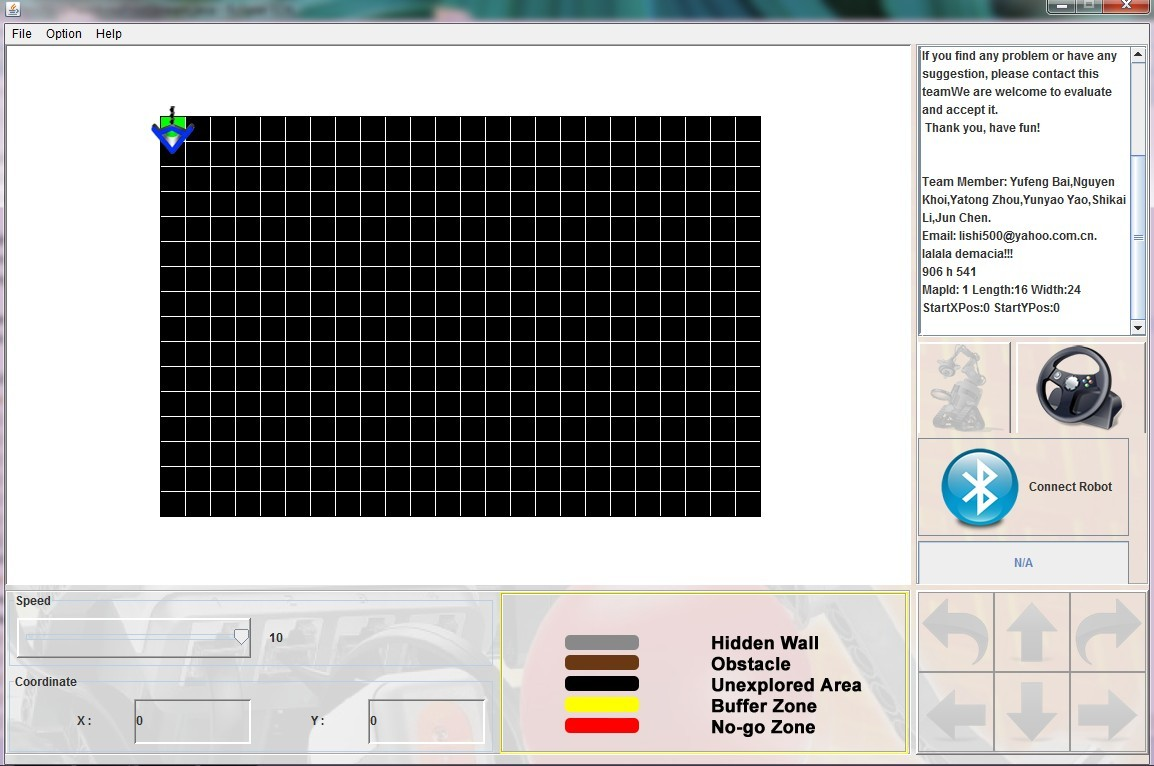
\includegraphics[width=11.20cm]{Map.jpg}
\end{center}
\begin{center}
\textbf {Figure 6.2: GUI WITH MAP} \\[0.3cm]
\end{center}
\section{Detailed Design of the User Interface}
\subsection{Create map}
The GUI includes a icon which is used to create a new map. When the user presses the "Create Map"  button, there is a window jumping out, the user is able to set the map size and the start point.
\begin{center}
 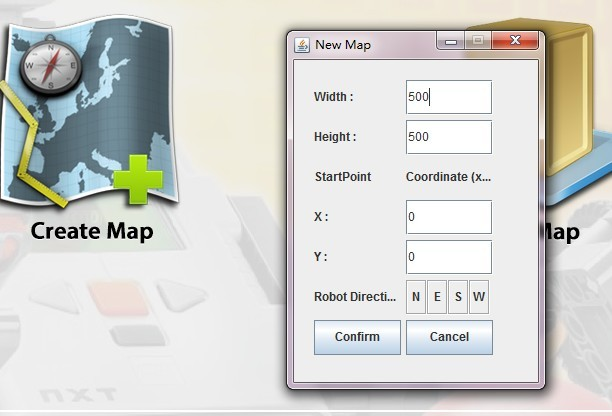
\includegraphics[width=9.20cm]{CreateNewMap.jpg}
\end{center}
\begin{center}
\textbf {Figure 6.3: Create Map} \\[0.3cm]
\end{center}
\subsection{Save map}
The GUI includes a icon which is used to save the map to a XML file. When the user presses the File menu and choose the save option, there is a window jumping out, the user is able to choose the file where they want to save.
\begin{center}
 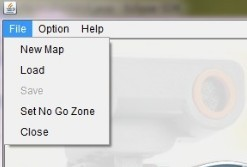
\includegraphics[width=9.20cm]{Menu_file.jpg}
\end{center}
\begin{center}
\textbf {Figure 6.4: Save Map} \\[0.3cm]
\end{center}
\subsection{Load map}
The GUI includes a icon which is used to load the map from a XML file. When the user presses that icon, there is a window jumping out, the user is able to choose the map from there.
\begin{center}
 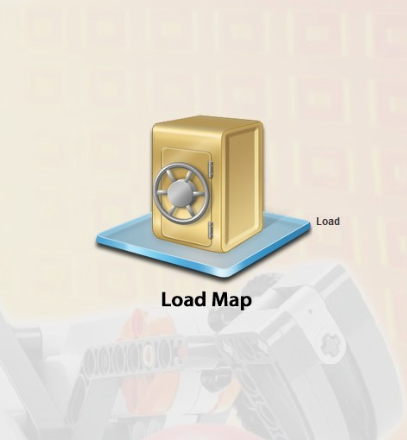
\includegraphics[width=8.20cm]{loadmap_quick}
\end{center}
\begin{center}
\textbf {Figure 6.5: Load Map Icon} \\[0.3cm]
\end{center}
\begin{center}
 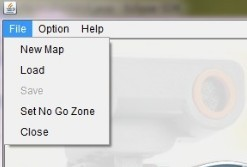
\includegraphics[width=8.20cm]{Menu_file.jpg}
\end{center}
\begin{center}
\textbf {Figure 6.6: Load MAP from menu bar} \\[0.3cm]
\end{center}
\begin{center}
 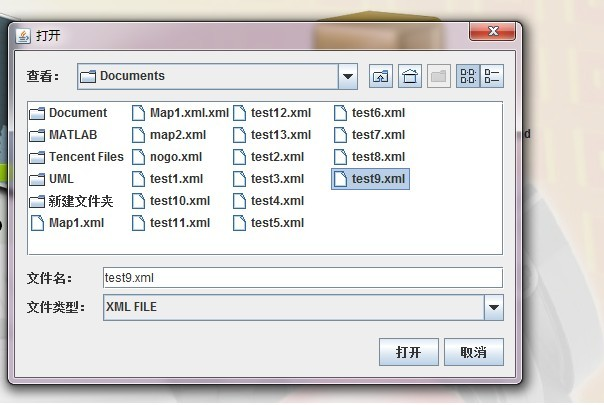
\includegraphics[width=8.20cm]{LoadMap.jpg}
\end{center}
\begin{center}
\textbf {Figure 6.7: Load Map} \\[0.3cm]
\end{center}
\subsection{Change the control mode}
The user is allowed to change the control mode by pressing the mode button. When the user presses the Auto mode button, there is a widget jumping out. Then if the user presses "yes", the robot changes to the Auto mode. The user is allowed to do the same operation to change to the Manual mode.  The Log information display which mode it is currently.
\begin{center}
 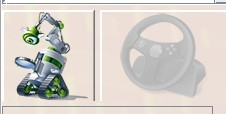
\includegraphics[width=10.20cm]{ControlModeAuto.jpg}
\end{center}
\begin{center}
\textbf {Figure 6.8: Change Mode} \\[0.3cm]
\end{center}
\begin{center}
 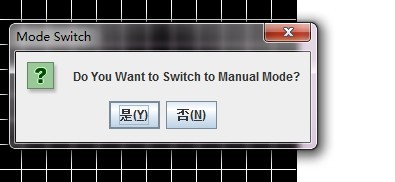
\includegraphics[width=11.20cm]{ModeSwitch.jpg}
\end{center}
\begin{center}
\textbf {Figure 6.9: Change Mode icon} \\[0.3cm]
\end{center}
\subsection{Connect to the robot via Blue-tooth}
Once the user press the control button on the robot, the robot will wait for blue-tooth connection. The user should press the blue-tooth connection button on the GUI to connect between the robot and the Host system.
 \begin{center}
 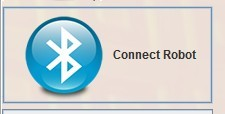
\includegraphics[width=10.20cm]{ConnectButton.jpg}
\end{center}
\begin{center}
\textbf {Figure 6.10: Blue-tooth Connection Button } \\[0.3cm]
\end{center}
\subsection{Demonstrate the Blue-tooth and battery status}
The Blue-tooth and battery status are displayed on the GUI, if the Blue-tooth loses the connection, the colour of the blue-tooth button will change to ashy and the log information board will demonstrate the lose information. The power of the battery is displayed by the percentage number and the colour of the battery bar will change along with the battery level.
 \begin{center}
 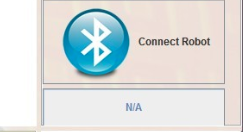
\includegraphics[width=11.20cm]{bluetooth_battery}
\end{center}
\begin{center}
\textbf {Figure 6.11: Blue-tooth and battery demonstration } \\[0.3cm]
\end{center}
 \begin{center}
 
\includegraphics[width=6.20cm]{connectionloss.jpg}
\end{center}
\begin{center}
\textbf {Figure 6.12: Blue-tooth Loss } \\[0.3cm]
\end{center}
\subsection{Control the moving direction of the robot}
The robot is able to be controlled by GUI when the robot is changed to the Manual mode. The user is allowed to press the arrows to move the robot. The robot is able to move forward, backward and rotate(include rotate 90 angles and rotate 360 angles). The moving direction controlling only can be used in Manual mode.
 \begin{center}
 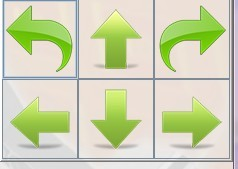
\includegraphics[width=11.20cm]{ControlButton.jpg}
\end{center}
\begin{center}
\textbf {Figure 6.13: Moving control} \\[0.3cm]
\end{center}
\subsection{Demonstrate the icon of the map}
The robot and map information are required to be displayed on the GUI. It is necessary to use different icons(colours) to demonstrate the different map information.
  \begin{center}
 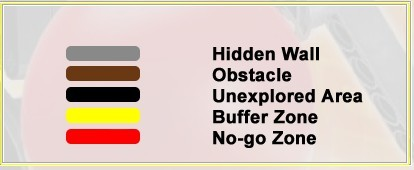
\includegraphics[width=11.20cm]{IconInformation.jpg}
\end{center}
\begin{center}
\textbf {Figure 6.14: Icon of the map} \\[0.3cm]
\end{center}
\subsection{Demonstrate information of the GUI on the log information board}
The Log Information board displays the information of the GUI. For example, the Log Information board demonstrates the version and the developers of the robot. If the user changes the control mode, the board displays which mode it is now. The board also is required to indicate the connection information.
  \begin{center}
 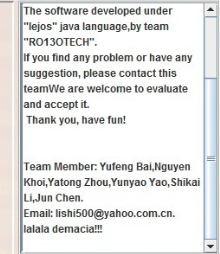
\includegraphics[width=11.20cm]{board}
\end{center}
\begin{center}
\textbf {Figure 6.15: The logging information} \\[0.3cm]
\end{center}
\subsection{Control the speed of the robot}
The GUI includes a speed bar and one specific number to control the speed of the robot. The host is allowed to change the speed of the robot by change the number of the bar. The larger number means the faster the robot is. If the number is zero, it means the robot stops immediately.
  \begin{center}
 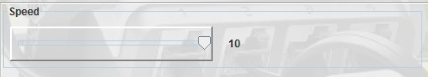
\includegraphics[width=8.20cm]{bar}
\end{center}
\begin{center}
\textbf {Figure 6.16: The speed controlling} \\[0.3cm]
\end{center}
\subsection{The location of the robot}
The GUI is required to display the specific location of the robot. The map is made up of a lot of pixels. The location of the robot is able to display by coordinate, which is more accurate. When the robot moves, the coordinate will changes immediately.
   \begin{center}
 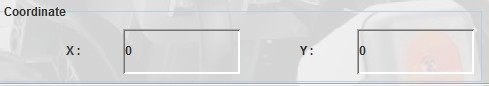
\includegraphics[width=8.20cm]{RobotCoordinate.jpg}
\end{center}
\begin{center}
\textbf {Figure 6.17: The coordinate of the robot} \\[0.3cm]
\end{center}
\subsection{Add "no-go" zones to the map}
Users can add "no-go" zones to the map by  pressing the Option menu and choose the Set No Go Zone option. Then users can use mouse clicks to set the size of the "no-go" zone. Also, users can redo or undo the setting of "no-go" zone.
  \begin{center}
 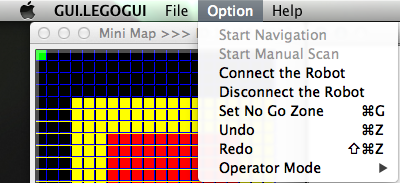
\includegraphics[width=11.20cm]{NoGoZoneOption.png}
\end{center}
\begin{center}
\textbf {Figure 6.18: Set No-go Zone Option} \\[0.3cm]
\end{center}
  \begin{center}
 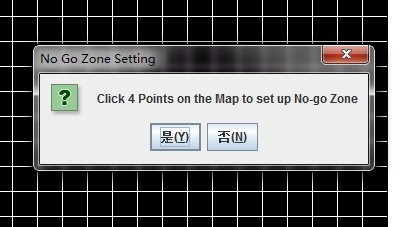
\includegraphics[width=11.20cm]{setNoGoZone1.jpg}
\end{center}
\begin{center}
\textbf {Figure 6.19: Set No-go Zone} \\[0.3cm]
\end{center}
  \begin{center}
 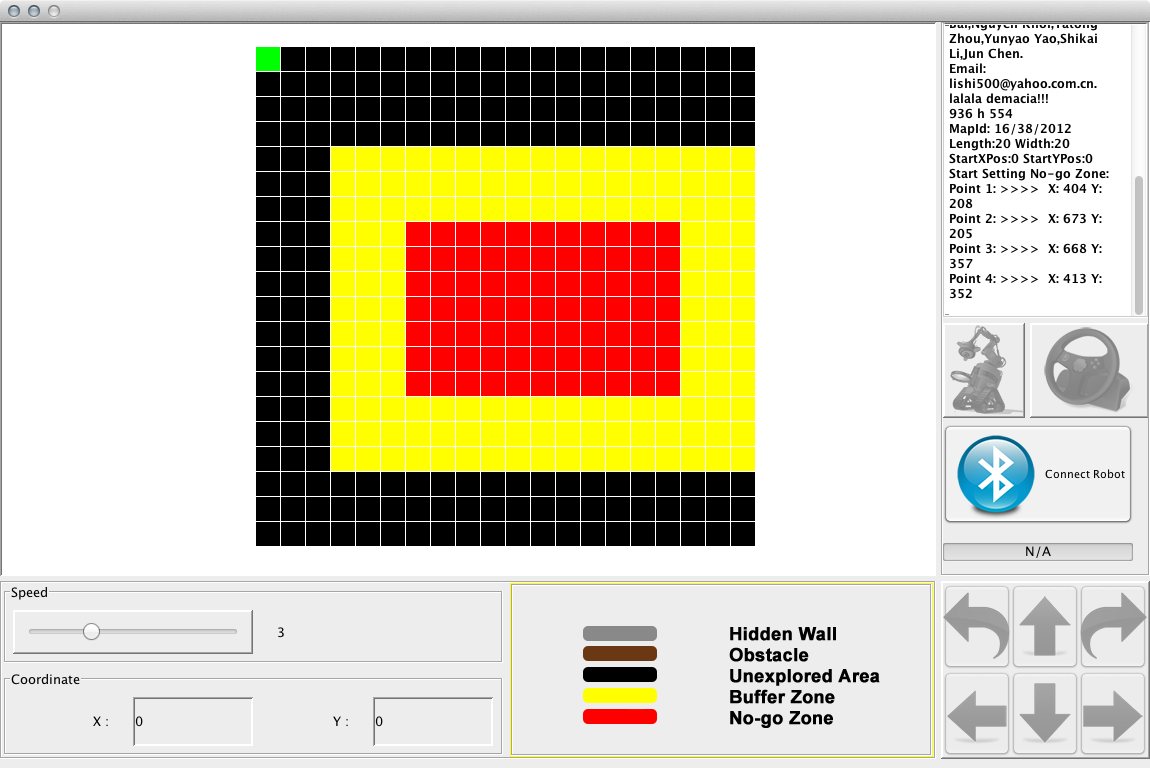
\includegraphics[width=10.20cm]{NoGoZone.png}
\end{center}
\begin{center}
\textbf {Figure 6.20: No-go Zone} \\[0.3cm]
\end{center}


%You have to present your user interface design from the following perspectives:
%? Screen Images: screenshots showing the interface from end users? perspec- tive.
%? Screen Objects and Actions: discussion of screen objects and the actions associated with those objects.
%? Report Forms: a description of major reports provided by the system, if any.
%Note: all the interface designs have to link to the user requirements and functional requirements in the SRS; all the interface images shall be num- bered.


% chapter Interface Design (end)
\pagebreak




\chapter{Resource Estimates} % (fold)
\label{cha:RE}
%A summary of computer resource estimates required for operating the system.%
The resource of the project is estimated according to the Project Description and the client's requirements in every week's meeting. All hardware and software which are used in the project are demonstrated below.
\section{Hardware}
\subsection{Robot}
Name: NXT Robot includes all components of the robot:
\begin{itemize}
\item LCD display - to display detail information of the robot
\item Control buttons - to control  robot and connect to the host machine.
\item Light sensor - to detect hidden walls
\item Ultrasonic sensor - to detect obstacles
\end{itemize}
Function: The robot is used to search the map and find all the obstacles, hidden walls and "no-go" zone. All operations are required to finish by controlling the robot.
\subsection{Host}
Name: PC\\
Function: The PC is required to demonstrate the searching information of the robot. PC is also used to control the robot on Manual Mode. The programs are uploaded to the robot from the PC.
\subsection{Connection}
Name: Blue-tooth and USB \\
Function: The Blue-tooth and USB are all used to connect with the robot. The USB is limited by the length of the cable. The Blue-tooth is limited by the uploading speed. In this project, the USB is used to upload the program and the Blue-tooth is used to implement the manual control.
\section{Software}
\subsection{Operation Environment}
Name: Mac, Linux and Windows\\
Function: This project is not providing the working environment. Any system is able to develop the programs for the robot.
\subsection{Developing language}
Name: Java SE 6, latex\\
Function: The codes are allowed to write in Java language, which is convenient to be read by any developers. The documents are required to write by Latex, then generating the PDF documents.
\subsection{Developing tool}
Name: Eclipse\\
Function: Eclipse is a better tool to make the program for this project. The Eclipse is used to write the operation commands for the robot and draw the GUI for this project.
\subsection{Robot Software}
Name: leJOS 0.9.1\\
 Function: The leJOS is used to control the robot and developing tool is required to support the leJOS 0.9.1.
 \subsection{Testing tool}
 Name: JUnit\\
 Function: The JUnit is used to debug the code.

% chapter Resource Estimates (end)
\pagebreak

\chapter{Definitions, Acronyms, and Abbreviations} % (fold)
\label{cha:DAA}
\section{Acronyms and Abbreviation}
\begin{center}
\begin{tabular}{|l|c|}
  \hline
  \textbf{Acronyms/Abbreviation} & \textbf{Description}\\
  \hline
  API		& Application Programmable Interface \\
  \hline
  BT		& Blue-tooth \\
  \hline
  GUI		& Graphical User Interface \\
  \hline
  PC		& Personal Computer\\
  \hline
  SRS	& Software Requirements Specifications \\
  \hline
  SPMP 	& Software Project Management Plan \\
  \hline
  UML	& Unified Modelling Language\\
  \hline
  USB	& Universal Serial Bus\\
  \hline
  XML 	& eXtensible Markup Language \\
  \hline
\end{tabular} \\[0.3cm]

\textbf {Table 1: Acronyms/Abbreviations} \\[0.3cm]
\end{center}
%Provide definitions of all terms, acronyms, and abbreviations used in SDD.%
\section{Definitions}
\begin{enumerate}
\item API: A set of classes and interfaces which are used to make the program for the robot include PC API and lejos API.\\
\item BT: A device to implement the wireless connection.\\
\item GUI: A interface which is generated on the PC is used to send the commands to the robot.\\
\item PC: A device which is used to make the program for the robot and build the GUI.\\
\item UML: A modelling language is used to build the diagrams for the project.\\
\item USB: A device to implement the wired connection.\\
\item XML: The data structure is used to store the map information.\\
\end{enumerate}
% chapter Definitions, Acronyms, and Abbreviations (end)
\pagebreak
% Appendices %
\newpage
\appendix

\pagebreak

\end{document}
